\section{Introduction}\label{sec:intro}
Deep neural networks (DNNs) have shown tremendous success in several computer vision tasks in recent years [\cite{resnet},\cite{schroff2015facenet},\cite{krizhevsky2012imagenet}]. However, seminal works on adversarial examples [\cite{goodfellow2014explaining}, ~\cite{szegedy2013intriguing}] have shown that DNNs are susceptible to imperceptible perturbations at input and intermediate layer activations. From an optimization perspective, they also showed that adversarial training can be used as a regularization approach while training deep networks.  The focus of adversarial training techniques has been to improve network robustness to gradient based adversarial perturbations. In this work, we propose a novel variant of adversarial training with a focus to improve regularization performance on test data.

% \begin{figure}[t!]
% \centering
% 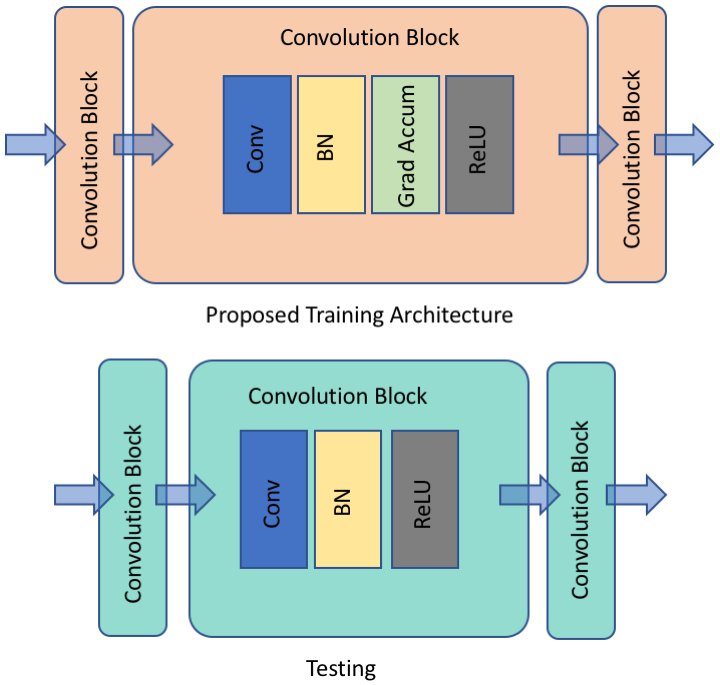
\includegraphics[width=0.35\textwidth, height=0.5\linewidth]{figure_approach.png}
% \caption{Proposed gradient accumulation layer (\textit{Grad Accum} in top row) for training deep neural network. During testing, gradient accumulation layers are turned off and it is a standard feed forward architecture.}
% \label{fig:approach}
% \end{figure}

%dropconnect  ~\cite{icml2013_wan13}, weight decay ~\cite{} have been proposed to regularize neural network training. 

%Adversarial examples are generated by adding small imperceptible structured noise to the input which leads to their misclassification by the network. They performed adversarial training for each layer by alternating between generating samples for each layer and updating the network parameters. However, generating adversarial examples for each layer is very expensive and can't be extended to very deep state-of-the-art networks such as ResNet ~\cite{resnet}. One of the key insights provided in the study, and which was not discussed in details, is that the improvement in classification performance is achieved only when adversarial examples are generated for each layer.

%The study further reported that improvement in performance and regularization is best achieved when hidden layers are also perturbed using adversarial gradients.

%One of the conclusions of the paper was that, using the fast gradient sign method, perturbation at the input layer performed comparable to perturbation at the hidden layers. 

%Recent works ~\cite{szegedy2013intriguing}, ~\cite{goodfellow2014explaining} have shown that adversarial training can act as regularization to the deep neural networks.

%Adversarial training leverages the susceptibility of deep neural networks to small imperceptible structured noise in the input to immunize them against adversarial examples and regularize training. ~\cite{szegedy2013intriguing} proposed a box constrained optimization formulation to perform adversarial training. However, their approach did not provide regularization beyond dropout. ~\cite{goodfellow2014explaining} proposed a fast gradient sign method to generate adversarial examples and an adversarial objective loss function to regularize DNN training. They observed that their adversarial training procedure adds regularization beyond dropout and also makes the network robust to adversarial examples. However, the analysis of adversarial training was limited to shallow networks since both the approaches are computationally expensive and can't be easily extended to very deep networks such as VGG or ResNet without significant computational overhead. 

%(~\cite{szegedy2013intriguing} requires solving box-constrained optimization problem while ~\cite{goodfellow2014explaining} requires additional forward and backward pass)

%Similarly, ~\cite{understandingAT} proposed an additional ascent-descent step to generate gradient direction that leads to maximum loss and used those gradients to perturb input data for adversarial training. However, adversarial examples are generated only at the input layer and such training procedure leads to marginal improvement in classification performance at test time. 
%However, L-BFGS algorithm is very expensive and it is difficult to perform large scale experiments using this approach. Moreover, the regularization demonstrated by the proposed approach did not improve beyond dropout in experiment evaluations. 
%All the previously proposed adversarial training approaches requires generating adversarial examples to augment the training through additional forward and backward pass or through some optimization procedure such as L-BFGS. Also these procedures are not very efficients for very large networks such as ResNet where generating additional examples for each layer and training network alternatively is not feasible during training process.

%drop out on large dataset's requires careful application of dropout layer.
%larger datasets and deeper network

%To best of our knowledge, this is first such study for such deep large neural networks. 

The proposed approach is efficient and simple to implement. It uses adversarial perturbations of intermediate layer activations to provide a stronger regularization compared to traditional techniques like Dropout (\citeauthor{srivastava2014dropout} \citeyear{srivastava2014dropout}). By generating the perturbations from a different class compared to the current input, we ensure that the resulting perturbations in the intermediate layers are directed towards an adversarial class. This forces the network to learn robust representations at each layer resulting in improved discriminability. Even though these perturbations are not adversarial at the input layer, we show that they are strongly adversarial when applied at the intermediate layers. 
%Despite not training the network with adversarial examples, we also observe an improved robustness of the deep network to such data. %\textbf{Our experiments show that perturbing intermediate layer activations throughout the network produces more immunity to adversarial inputs than perturbing just the input layer and hence achieves better regularization.}

%experiment to show suboptimality of gradient direction at input layer
The proposed regularization approach does not add any significant overhead during training and thus can be easily extended to very deep neural networks, as shown in our experiments. Our approach complements dropout and achieves regularization beyond dropout. It avoids over-fitting and generalizes well by achieving significant improvement in performance on the test set. We show that the trained network develops robustness against adversarial examples even when it is not explicitly trained with adversarial inputs. While previous works have focused on generating adversarial perturbations for standalone images, our work focuses on using these to efficiently regularize training. We perform several ablative experiments to highlight the properties of the proposed approach and present results for very deep networks such as VGG~\cite{vgg}, ResNets~\cite{resnet} and state of the art models such as WideResNets \cite{wideresnet} on CIFAR-10, CIFAR-100 and ImageNet datasets.


%Deep Neural networks have produced state of the art results for variety of machine learning tasks. However, recent studies [] have shown that they are not locally stable (due to existance of blind spots) and even a small imperceptible perturbations when added to the input can lead to misclassification by neural networks.

%Deep neural networks have shown tremendous success in variety of machine learning tasks. However, recent studies [] have shown that they are not locally stable (due to existance of blind spots) and even a small imperceptible perturbations when added to the input can lead to misclassification by neural networks. [] proposed a fast-sign gradient method to generate these adversarial examples, while [] proposed iterative genetic algorithm based approach to generate fooling images .... Harnessing these adversarial examples is an active area of research and recent works by [] have shown that these adversarial training can improve not only the stability of neural networks against the adversarial examples but also obtain marginal improvement in test performance. 

%In this work, we investigate the use of these adversarial perturbations directly during the training phase without explicitly generating adversarial examples. We propose a new layer - Adversarial Layer - which can be easily incorporated into deep neural network training without any overhead.

%The proposed layer perturbs the internal representation of the network using adversarial gradients and thus forcing network to learn better representation that separates the classes leading to improved performance. 

%- A very simple training strategy which caches intermediate gradient without having to explicitly generate adversarial examples for each layer. No need for alternative training or explicitly generating adversarial examples for training.

%- scalability - our approach allows to train very large networks such as Resnet-150 efficiently.

%- efficient as no need to perform extra backward and forward pass.

%- regularization benefits as shown with adversarial training. We show that adversarial training can provide an additional regularization benefit beyond that provided by using dropout

%- this has a connection with hard-mining where the examples are generated implicitly rather explicitly. Mining is performed in intermediate layers as part of the forward pass.

%- [] investigates strong connection between regularization and robust optimization. They propose an approach to perturb input image within a ball of radius of r using the direction which leads to maximum loss. Since the test examples and adversarial examples both occur close to training set, they showed marginal improvement in test performance and more robustness to adversarial test set.

%- adversarial training provides regularization. It even provides regularization on top of dropout \cite{[goodfellow2014explaining]}

%- Proposed approach makes the trained network hard to generate adversarial examples. 

%- we didn't have to modify the loss function as done in \cite{goodfellow2014explaining} to regularize training. These layers acts as regularizer during training

%- Even though the gradients from previous samples are not strong adversary to the input image, due to shared representation in the feature space, their gradients in feature space act as strong adversary.

%- Our work built on preliminary results of \cite{goodfellow2014explaining} where perturbing internal layers of CNNs achieves higher performance. However, their approach involved generating adversarial examples for each layer separately and training which is a very tedious process. Our approach allows to perform adversarial training directly by caching the gradients of samples and then using them directly to perturb internal CNN layers for adversarial training. Our approach generalize to very large neural networks such as Resnet 150 without any additional overhead in training at the same time achieves significant improvement in performance. 

%- Position of these gradient layers has impact on the how well they regularize training. 

%- By perturbing the shared input representation of feature space, we are forcing network to pick better representations which distinguishes the classes. 

%- why adversarial training doesn't work when perturbing only top layers and bottom layers. 

%- normalize gradients to the range of the layers value. Perturbations according to the range of the layer. We observed significant drop in performance when we fixed epsilon without scaling.


%*one experiment we should do is to add gradients from previous sample to input image and test it

%- classifier performance depends on distinguishability between classes \cite{fawzi2015analysis}. 